% 
% Annual Cognitive Science Conference
% Sample LaTeX Paper -- Proceedings Format
% 

% Original : Ashwin Ram (ashwin@cc.gatech.edu)       04/01/1994
% Modified : Johanna Moore (jmoore@cs.pitt.edu)      03/17/1995
% Modified : David Noelle (noelle@ucsd.edu)          03/15/1996
% Modified : Pat Langley (langley@cs.stanford.edu)   01/26/1997
% Latex2e corrections by Ramin Charles Nakisa        01/28/1997 
% Modified : Tina Eliassi-Rad (eliassi@cs.wisc.edu)  01/31/1998
% Modified : Trisha Yannuzzi (trisha@ircs.upenn.edu) 12/28/1999 (in process)
% Modified : Mary Ellen Foster (M.E.Foster@ed.ac.uk) 12/11/2000
% Modified : Ken Forbus                              01/23/2004
% Modified : Eli M. Silk (esilk@pitt.edu)            05/24/2005
% Modified : Niels Taatgen (taatgen@cmu.edu)         10/24/2006
% Modified : David Noelle (dnoelle@ucmerced.edu)     11/19/2014

%% Change "letterpaper" in the following line to "a4paper" if you must.

\documentclass[10pt,letterpaper]{article}

\usepackage{cogsci}
\usepackage{pslatex}
\usepackage{apacite}
\usepackage{url}
\usepackage{graphicx}
\usepackage{caption}
\usepackage{subcaption}
\usepackage{listings}

\usepackage{amsmath}
\usepackage{amssymb}
\usepackage{wrapfig}


\newcommand*\diff{\mathop{}\!\mathrm{d}}
\newcommand{\denote}[1]{\mbox{ $[\![ #1 ]\!]$}}
\newcommand{\tableref}[1]{Table \ref{#1}}
\newcommand{\figref}[1]{Figure \ref{#1}}
\newcommand{\appref}[1]{Appendix \ref{#1}}
\newcommand{\sectionref}[1]{Section \ref{#1}}


\graphicspath{{img/}}

\title{``Not unreasonable'': The logic of double negation in natural language}
 
\author{{\large \bf Michael Henry Tessler (mhtessler@stanford.edu)} \\
  Department of Psychology, Stanford University 
  \AND {\large \bf Michael Franke (mchfranke@gmail.com)} \\
  Department of Linguistics, University of T\"{u}bingen}


\begin{document}

\maketitle


\begin{abstract}

If ``John is not unhappy'', does that mean that he's happy? 
In logic, two negatives make a positive, but the same does not seem to hold in natural language. 
Instead, antonyms and their negations appear to partition the underlying semantic scale in an ordering: ``unhappy'' $<$ ``not happy'' $<$ ``not unhappy'' $<$ ``happy'' \cite{Horn1989:Natural, Krifka2007:Negated-antonyms}. 
We show how this semantic ordering falls out of an information-theoretic model of adjective interpretation, without assuming that ``unhappy'' $<$ ``happy''.
We then empirically investigate the semantic ordering, finding that the ordering appears when participants are fully aware of the utterances a speaker could say for antonym pairs defined by morphological negation (``[un]happy''); the explicit presentation of alternatives is not necessary for the analogous ordering of antonym pairs of distinct lexical items (``tall'' / ``short''). 
These findings suggest a model of interpretation where listeners maintain uncertainty about the parsing of an utterance involving multiple negations.


\textbf{Keywords:} 
semantics; pragmatics; Rational Speech Act; Bayesian cognitive model; adjectives
\end{abstract}


\section{Introduction}

Every introductory logic student will tell you that two negations cancel each other out: A ``not ungreen'' field is green.
Yet in natural language, there exist multiple, seemingly distinct ways of conveying negation.  
Opposites can be arrived at by altering the morphology of a word: ``un-'' + ``happy'' $\rightarrow$ ``unhappy''.
In addition, a modifier that induces negation can be employed: ``not happy''.
Contra logic, however, these two ways of employing negation \emph{do not} cancel each other out: someone ``not unhappy'' is not necessarily happy. 	
As \citeA{Jespersen1924} noted:
%
\begin{quote}
%The two negatives do not exactly cancel one another...; 
the longer expression is always weaker: ``this is not unknown to me'' or ``I am not ignorant of this'' means \emph{I am to some extent aware of it}, etc.
\end{quote}
%

Competing intuitions arise concerning the logic of double negation in natural language. 
\citeA{Horn1991:Duplex, Horn1993:Economy} provides an explanation wherein  ``not unhappy'' is provided a restricted interpretation via its literal meaning and pragmatic competition with ``happy''. 
Contra intuition, this would result an interpretation of ``not unhappy'' that is neutral or indifferent, which contradicts intuitions that suggest ``not unhappy'' is a slightly positive state \cite<e,g.,>{Krifka2007:Negated-antonyms}.
Some have suggested that ``not happy'' is an alternative that should enter into the division of pragmatic labor \cite{Blutner2004:pragmatics}, but the pragmatic logic would contextually strength ``not happy'' is heretofore unclear \cite{Krifka2007:Negated-antonyms}. 

Theorists' intuitions further conflict on the difference in meaning between ``not happy'' and ``unhappy''.
\citeA{Jespersen1917:Negation} and \citeA{Blutner2004:pragmatics} believe the two are basically identical in meaning. 
\citeA{Horn1989:Natural} and \citeA{Krifka2007:Negated-antonyms} disagree, citing examples found on the internet such as ``It's an absolutely horrible feeling to be unhappy, and I don't even think I was unhappy, just not happy, if you know what I mean.''

These two issues motivate our current approach.
First, competing intuitions concerning the meaning of modifier negation (``not happy'') and morphological negation (``unhappy'') suggest that empirical data should be consulted before further theorizing about pragmatic mechanisms.
Second, the fact that the logic surrounding the pragmatic strengthening of modifier negation (``not happy'') in the context of alternative utterances is not clear suggests that the logic of double negation may benefit from a formal modeling approach. 
Thus, we take an empirically-driven, formal modeling approach in this paper.
We first elaborate a computational model of adjective interpretation to include antonyms and their negations, which we collectively refer to as \emph{antonym quartets}: adjectives (e.g., ``tall''), their antonyms (e.g., ``short''), and the negations of each (``not tall'', ``not short'').
In Experiments 1 \& 2, we investigate the hypothesized ordering of antonym quartets for antonyms with distinct lexical entries (e.g., ``tall'' and ``short'') and antonyms constructed from a morphological change (e.g., ``happy'' and ``unhappy'').
We conclude by revising the model in light of the empirical data. 


\section{Computational model}

Gradable adjectives (e.g., ``tall'', ``happy'') convey the value along a scale (e.g., \emph{height}, \emph{happiness}) for some referent $x$ is above or below some contextually-specified threshold: $\denote{tall} = \emph{height}(x) > \theta$; $\denote{short} = \emph{height}(x) < \theta$.
\citeA{Lassiter2013} provided a probabilistic pragmatics model that constrains the threshold $\theta$ relative to a context, formalized by a prior distribution over the value of the scalar degree $x$.  
%
\begin{align}
L_{1}(x, \theta \mid u) &\propto S_{1}(u \mid x, \theta) \cdot P(x) \cdot P(\theta) \label{eq:L1} \\
S_{1}(u \mid x, \theta) &\propto \exp{(\alpha_1 \cdot \ln {L_{0}(x \mid u, \theta)} - \text{cost}(u))} \label{eq:S1}\\
L_{0}(x \mid u, \theta) &\propto {\delta_{[\![u]\!](x, \theta)} \cdot P(x)} \label{eq:L0}
\end{align}
%
Equations \ref{eq:L1}-\ref{eq:L0} comprise a Rational Speech Act (RSA) model, a recursive Bayesian model wherein a pragmatic listener $L_1$ tries to resolve the intended meaning of an utterance $u$ by combining their prior beliefs $P(x)$ with the generative process of the utterance, a speaker model $S_1$ \cite<for a review, see>{Goodman2016:RSA}.
The speaker model $S_1$  is an approximately rational Bayesian agent trying 
to inform a naive listener $L_0$ (Eq.~\ref{eq:L0}) about the state of the world $x$.
In the context of adjective interpretation, the state of the world is given by the value of the scalar degree $x$ (e.g., the height of the referent).
The literal listener updates their prior beliefs $P_(x)$ via an utterance's literal meaning $[\![u]\!](x)$, the threshold function described above.
The pragmatic listener has uncertainty about $\theta$, which comes from an uninformed prior and is resolved by jointly reasoning about the likely states of the world $P_(x)$ (e.g., possible heights) and the likelihood that a speaker would say the adjective given a state and a threshold $S(u \mid x, \theta)$.

The proportionality in Eq.~\ref{eq:S1} implies normalization over a set of alternative utterances (potentially differentiated by their cost). 
Formal models of adjective interpretation (including an alternative model proposed by \citeNP{Qing2014:Adjectives}) have so far restricted the set of alternative utterances to be only an adjective (e.g., either ``tall'' or ``short'') and an information-less, null utterance. 
In order to better understand the information-theoretic, pragmatic logic of antonyms and negation, we eschew the null utterance and introduce antonyms in the alternative set, as well as their logical negation (glossed as modifier negation, e.g., ``not tall'' and ``not short''). 
Following standard approaches in formal semantics, antonyms are given their own thresholds ($\theta_-$), so Eq.~\ref{eq:L1} becomes:
%
\begin{align}
L_{1}(x, \theta_+, \theta_- \mid u) &\propto S_{1}(u \mid x, \theta_+, \theta_-)  P(x)  P(\theta_+)  P(\theta_-) \label{eq:L1a}
\end{align}
\subsection{Model behavior}


\section{Experiment 1: Measuring the ordering}
\subsection{Methods}
\subsubsection{Participants}

We recruited 120 participants from Amazon's Mechanical Turk (MTurk). 
This number was arrived it with the intention of getting approximately 25 ratings for each unique item in the experiment.
In all experiments, participants were restricted to those with U.S. IP addresses and who had at least a 95\% work approval rating. 
The experiment took on average N minutes and participants were compensated \$N for their work.

\subsubsection{Materials}

We used adjective quartets composed of positive-form gradable adjectives (\emph{POS}; e.g., ``happy''), their antonym (\emph{ANT}; e.g., ``unhappy''), and their respective negations (\emph{NEG POS}, ``not happy''; \emph{NEG ANT} ``not unhappy''); we refer to these four \emph{sentence types} collectively as an \emph{antonym quartet}.
Antonyms were either created by morphological negation (\emph{morphological antonyms}; e.g., ``unhappy'' for ``happy'') or were distinct lexical entries (\emph{lexical antonyms}; e.g., ``short'', for ``tall'').
All adjectives were individual-level predicates that applied to people; items were constructed from an informal survey of the linguistics literature and taken from list of ``common opposites'' available online\footnote{http://www.enchantedlearning.com/wordlist/opposites.shtml} (for a full list, see \tableref{tab:items}.

\begin{table}[b]
\centering
\begin{tabular}{l|l}
\emph{Morphological antonyms}     & \emph{Lexical antonyms}    \\ 
\hline
happy, unhappy             & tall, short         \\
intelligent, unintelligent & rich, poor          \\
polite, impolite           & fat, skinny         \\
interesting, uninteresting & hard-working, lazy  \\
attractive, unattractive   & brave, cowardly     \\
successful, unsuccessful   & beautiful, ugly     \\
honest, dishonest          & wise, foolish       \\
educated, uneducated       & proud, humble       \\
friendly, unfriendly       & strong, weak        \\
mature, immature           & loud, quiet        
\end{tabular}
\caption{Antonym pairs used in Experiments 1 \& 2}
\label{tab:items}
\end{table}


\subsubsection{Procedure}

On each trial, participants read a statement introducing a character using a gradable adjective in one of the four \emph{sentence types} (e.g., ``Greg is \{POS, ANT, NEG POS, NEG ANT\}'').
Participants were asked to interpret the statement by placing the character on a scale from ``the most POS person'' to ``the most NEG person'', using a slider bar (\figref{fig:expt1}).
Participants completed 16 trials; each used a different adjective quartet.
Throughout the course of the experiment, participants saw 2 of each \emph{sentence type} with both \emph{lexical} and \emph{morphological} antonym quartets. 

\begin{figure}[t]
	\centering
	\begin{subfigure}[t]{0.5\textwidth}
		\centering
		\frame{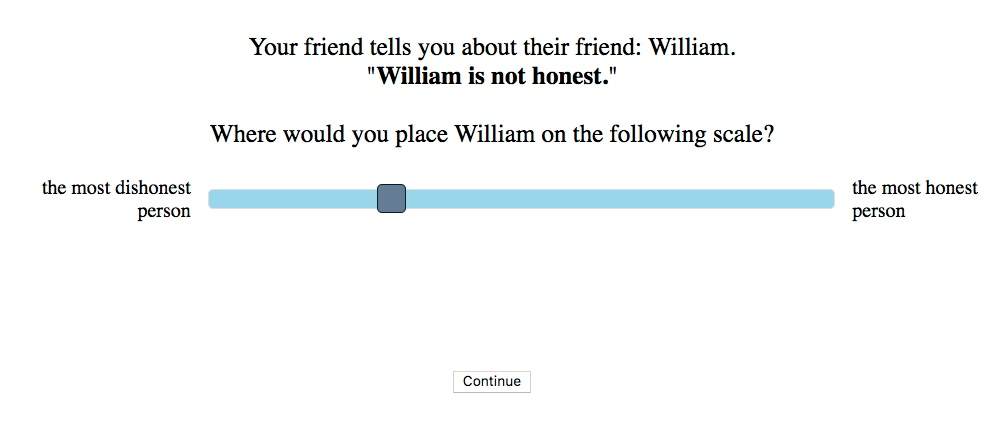
\includegraphics[width=\textwidth]{expt1.jpeg}}
		\caption{Experiment 1}\label{fig:expt1}		
	\end{subfigure}%
	\quad
	\begin{subfigure}[t]{0.5\textwidth}
		\centering
		\frame{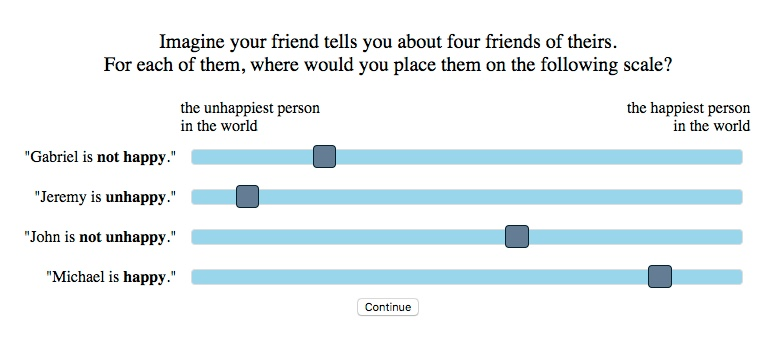
\includegraphics[width=\textwidth]{expt2.jpeg}}
		\caption{Experiment 2}\label{fig:expt2}
	\end{subfigure}
	\caption{Example experimental trials.}\label{fig:expt-procedure}
\end{figure}


\subsection{Results}

X participants were excluded for self-reporting a native language other than English. 


\section{Experiment 2: Explicit alternatives}
This experiment was designed in order to test the influence of salient alternatives on the hypothesized semantic ordering for antonym quartets.

\subsection{Methods}

\subsubsection{Participants}

We recruited 50 participants MTurk.
This number was arrived it with the intention of getting approximately 25 ratings for each unique item in the experiment.
The experiment took on average N minutes and participants were compensated \$N for their work.


\subsubsection{Materials and Procedure}
The experimental materials were the same as in Expt.~1. 
The procedure differed in that participants saw and rated all four sentence types simultaneously (\figref{fig:expt2}). 
In addition, the endpoints of the slider bars were relabeled to ``the most \{\emph{POS}, \emph{ANT}\} person \emph{in the world'}'; excluding the ``in the world'' phrase leads to a salient interpretation of the endpoints as indicating ``the most \emph{POS} person (of these four)''.

\subsection{Results}

\section{Discussion}

\section{Acknowledgments}


\bibliographystyle{apacite}

\setlength{\bibleftmargin}{.125in}
\setlength{\bibindent}{-\bibleftmargin}

\bibliography{negant}


\end{document}
